% Prepared by Calvin Kent
%
% Assignment Template v19.02
%
%%% 20xx0x/MATHxxx/Crowdmark/Ax
%
\documentclass[12pt]{article} %
\usepackage{CKpreamble}
\usepackage{CKassignment}
\usepackage{tkz-euclide}
\usepackage{physunits}
\usepackage{physics}
\usepackage{lmodern}
\usepackage{microtype}
\usepackage{upgreek}
\usepackage[misc]{ifsym}
\title{Physics 11 Test 1 \\ \textbf{Time : 1.5 hrs}}
\date{2021\\ August}
\author{Abdullah Zubair}

%%% Maths and science packages

\usepackage{amsmath,amsthm,amssymb}
\usepackage{pgfplots}
	\usetikzlibrary{
		calc,
		patterns,
		positioning
	}
	\pgfplotsset{
		compat=1.16,
		samples=200,
		clip=false,
		my axis style/.style={
			axis x line=middle,
			axis y line=middle,
			legend pos=outer north east,
			axis line style={
				->,
			},
			legend style={
				font=\footnotesize
			},
			label style={
				font=\footnotesize
			},
			tick label style={
				font=\footnotesize
			},
			xlabel style={
				at={
					(ticklabel* cs:1)
				},
				anchor=west,
				font=\footnotesize,
			},
			ylabel style={
				at={
					(ticklabel* cs:1)
				},
				anchor=west,
				font=\footnotesize,
			},
			xlabel= $t$,
			ylabel=$\vec d (\m \tx{[East]})$
		},
	}
	\tikzset{
		>=stealth
	}

%%% Tables and figures packages

\usepackage{float}
\usepackage{caption}
	\captionsetup{
		format=plain,
		labelfont=bf,
		font=small,
		justification=centering
	}
	
%%% Numbers and sets

\newcommand{\E}{\mathrm{e}}

\newcommand{\tx}[1]{\text{#1}}

\begin{document}
    \pagenumbering{arabic}
    % Start of class settings ...
    \renewcommand*{\coursecode}{Test} % renew course code
    \renewcommand*{\assgnnumber}{1} % renew assignment number
    \renewcommand*{\submdate}{August 26, 2021} % renew the date
    \renewcommand*{\studentfname}{Abdullah} % Student first name
    \renewcommand*{\studentlname}{Zubair} % Student last name
    %\renewcommand*{\studentnum}{SNumber} % Student number

    \renewcommand\qedsymbol{$\blacksquare$}
    \setfigpath
    % End of class settings 
    \pagestyle{crowdmark}
    \newgeometry{left=18mm, right=18mm, top=22mm, bottom=22mm} % page is set to default values
    \fancyhfoffset[L,O]{0pt} % header orientation fixed
    % End of class settings
    %%% Note to user:
    % CTRL + F <CHANGE ME:> (without the angular brackets) in CKpreamble to specify graphics paths accordingly.
    % The command \circled[]{} accepts one optional and one mandatory argument.
    % Optional argument is for the size of the circle and mandatory argument is for its contents.
    % \circled{A} produces circled A, with size drawn for letter A. \circled[TT]{A} produces circled A with size drawn for TT.
    % https://github.com/CalvinKent/My-LaTeX
    %%%
    % Crowdmark assignment start


    %%%%%%%%%%%%%%%%%% PROBLEMS IDEAS %%%%%%%%%%%%%%%%%%%%%%%%%%%%%%%%%%%%%%%%%
	%% --> Half circle problem
    %% --> System of equations
    %% --> Comparing two motions, time difference
    %% --> Relative vector problem with at least 4 points
	%% --> REDO Q8 from review and this time ask him to compute the speed required.
	%% --> Problem related to question 8 from HW3 to test him


	\maketitle
	\section{Preamble}
	This is a test covering what we have learnt so far in lecture, that being Sections 1,2,3. The time expected to complete this test is just under an hour and half granted that the student is adequately prepared. Throughout the test, the student \emph{must show all work} to receive full marks.
	\section{Allowed Aids}
	The following aids are allowed on the Test
	\begin{itemize}
		\item Pencil, Pen, Eraser, Ruler, Protractor, Spare sheets of \textbf{blank} paper.
		\item Reference sheet \textbf{(FROM WEBSITE ONLY)}
		\item Basic scientific calculator
	\end{itemize}
	\section{Restrictions:}
	The student is not allowed to communicate with any outside source, nor allowed to access any external aid on the internet,etc. The student may ask the instructor (ME) any questions or confusions but is advised to do so only when all else has failed due to the time constraints.
	\section{Name and Date:}
	Print your name and todays date below;\\


	\begin{center}
	\noindent\begin{tabular}{ll}
		\makebox[3in]{\hrulefill} & \makebox[3in]{\hrulefill}\\
		Name & Date\\[8ex]% adds space between the two sets of signatures
	\end{tabular}
	\end{center}
	\newpage

\begin{qstn}[1]
	Answer the following True / False questions \textbf{(Assume [North],[East] is positive)}
	\begin{enumerate}
		\item The maximum height I can jump on a trampoline is $d = 5000\m$. I jump $3$ times on the trampoline and the time elapsed was $\Delta t = 20\s$. (\textbf{Assume} that a \emph{single jump} means I reached my maximum height \textbf{and} landed back on the trampoline)
			\begin{enumerate}[label = (\alph*)]
				\item My average velocity relative to the trampoline was $\vec v_{av} = +1700 \m / \s$. (T / F)
				\item My average speed was $v_{av} = 1.5 \km / \s$. (T / F)
			\end{enumerate}


		\item Suppose that relative to the center of a field, a batsmen stands at $\vec d_i = 50\m$[East]. The batsmen bats a baseball at an average velocity of $\vec v_{av} = 350 \m / \s$[West]. The time elapsed was $\Delta t = 15\s$.
			\begin{enumerate}[label = (\alph*)]
				\item $\vec d_f = 5200 \m$[East] is the final position vector. (T / F)
				\item The magnitude of the average velocity is equal to the average speed. (T / F)
			\end{enumerate}


		\item Consider the Moon orbiting the Earth
			\begin{enumerate}[label = (\alph*)]
				\item The average velocity of the Moon is \emph{always non-zero}. (T / F)
				\item The average speed of the Moon is \emph{always non-zero}. (T / F)
			\end{enumerate}
		
		
		\item Consider the equation of motion of \textcolor{blue}{Car A :} \textcolor{blue}{$x = -\frac{3}{2}t  + 12$} and \textcolor{red}{Car B :} \textcolor{red}{$x = \frac{7}{2}t - 7$}
			\begin{enumerate}[label = (\alph*)]
				\item Car $A$ has a greater average velocity than Car $B$. (T / F)
				\item Car $B$ is initially [East] relative to the reference point. (T / F)
				\item Car $A$ is initially [West] relative to the reference point. (T / F) 
				\item Both drivers experienced uniform motion. (T / F)
				\item Car $A$ and Car $B$ will meet at $t = 4\s$. (T / F)
			\end{enumerate}
		

		\item I kick a soccer ball at an average speed $v_{av}$ and it takes $\Delta t$ seconds to reach a distance of $d$ meters.
			\begin{enumerate}[label = (\alph*)]
				\item Kicking the soccer ball at $2v_{av}$ will allow it to travel $\frac{d}{2}$ meters in $\Delta t$ seconds. (T / F)
				\item Kicking the soccer ball at $\frac{v_{av}}{2}$ implies that it would take $2\Delta t$ seconds to travel $d$ meters. (T / F)
			\end{enumerate}
	
	\end{enumerate}

\end{qstn}
	

\begin{qstn}[2]
Answer the following multiple choice questions. \emph{Refer to the plot below for all Q1,Q2}.
		\begin{center}
			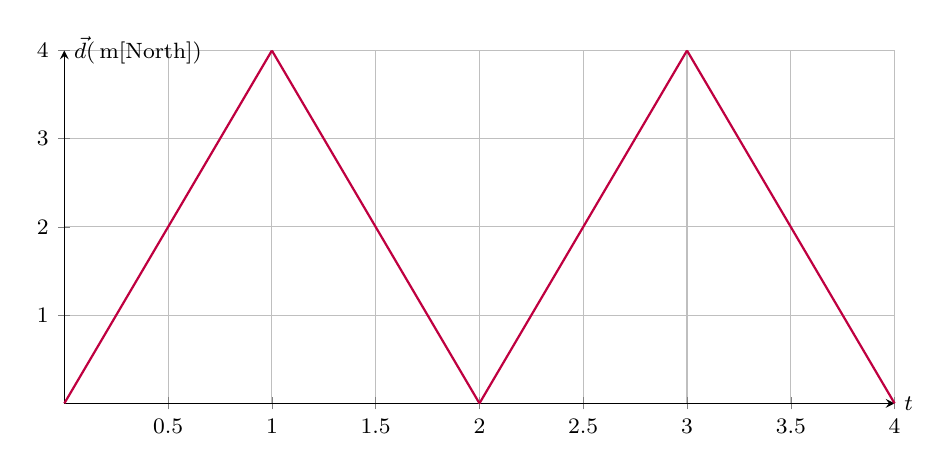
\begin{tikzpicture}
			\begin{axis}[
				my axis style,
				width=\textwidth,
				height=.5\textwidth,
				ylabel=$\vec d (\m \tx{[North]})$,
				grid
			]
			
			\addplot[
				domain=0:1,
				thick,
				purple,
				-
			]
			{4*x};
		
			\addplot[
				domain=1:2,
				thick,
				purple,
				-
			]
			{-4*x + 8};

			\addplot[
				domain=2:3,
				thick,
				purple,
				-
			]
			{4*x - 8};
		
			\addplot[
				domain=3:4,
				thick,
				purple,
				-
			]
			{-4*x + 16};
			
			\fill[
				black
			];
			
			\end{axis}
			\end{tikzpicture}
		\end{center}
	\begin{enumerate}
		\item Which of the following scenarios best describe the motion depicted in the plot,

			\begin{enumerate}[label = (\alph*)]
				\item A ball rolling [North] across a flat road
				\item A sprinter running on a circular track.
				\item A man jumping on a trampoline.
			\end{enumerate}


		\item Which of the following statements are correct about the plot?
			\begin{enumerate}[label = (\alph*)]
				\item The body experienced uniform motion within the time interval $[1,2]$.
				\item The body experienced uniform motion within the time interval $[0,4]$
				\item Within the time interval $[0,2]$, the average velocity was $\vec v_{av} = +0 \m / \s$.
				\item Within the time interval $[2,3]$, the average velocity was $\vec v_{av} = +4 \m / \ s$.
				\item The average speed within the time interval $[0,4]$ was $v_{av} = 4 \m / \s$.
			\end{enumerate}

		
		\item I label three points on a straight line, $F$, $G$, $H$. Which of the following statements are true?
			\begin{enumerate}[label = (\alph*)]
				\item $\vec d_{FG} = \vec d_{GF} + \vec d_{GH}$
				\item $\vec d_{HF} = (-\vec d_{FG}) + (-\vec d_{HG})$
				\item $\vec d_{FH} = (-\vec d_{GF}) + (-\vec d_{HG})$
				\item $-\vec d_{FG} = \vec d_{GH} + \vec d_{HG}$
			\end{enumerate}
	\end{enumerate}
	
\end{qstn}

\begin{qstn}[3]
Covert the following units to $\km / \h$. 
\begin{enumerate}[label = (\alph*)]
	\item $44200 \m / \s$
	\vspace*{5cm}

	\item $66 \km / \s$
	\vspace*{5cm}

	\item $5512 \inch / \Min$
\end{enumerate}


\end{qstn}

\begin{qstn}[4]
	Compute the \textbf{displacement} (or \emph{net} displacement) given the position vectors. Assume that the reference point is $(0,0)$ for \emph{all} vectors.
    \begin{enumerate}[label=(\alph*)]
        \item $\vec d_1 = 514 \tx{\m}[\tx{West}]$, $\vec d_2 = 332 \tx{\m}[\tx{West}]$
         \vspace*{4cm}
        \item $\vec d_1 = 51 \tx{\m}[\tx{S}]$, $\vec d_2 = 33 \tx{\m}[\tx{S}]$, $\vec d_3 = 27 \tx{\m}[\tx{N}]$, $\vec d_4 = 93 \tx{\m}[\tx{N}]$,$\vec d_5 = 298 \tx{\m}[\tx{S}]$, $\vec d_6 = 432 \tx{\m}[\tx{N}]$
        \vspace*{4cm}
        \item $\vec d_1 = 4\tx{\m}[\tx{East}]$, $\vec d_2 = 4\tx{\m}[\tx{West}]$, $\vec d_3 = 4\tx{\m}[\tx{North}]$, $\vec d_4 = 4\tx{\m}[\tx{East}]$
		\vspace*{5cm}
    \end{enumerate}
\end{qstn}




\begin{qstn}[5]
	Determine the sum/difference of the following vectors \textbf{\emph{geometrically}}. Use the $x-$dimensional coordinate system.
	\begin{enumerate}[label=(\alph*)]
		\item $\vec A = +2$, $\vec B = -8$ $$\vec A + \vec B$$
		\vspace*{3cm}
		\item $\vec A = +4$, $\vec B = -3$, $\vec C = +10$, $\vec D = -12$, $\vec E = -13$, $\vec F = +20$   $$(\vec A + \vec B) - (\vec C - \vec D) + (\vec E - \vec F)$$

	\end{enumerate}
\end{qstn}




\begin{qstn}[6]
	Suppose a train took the following route the other day to the following cities; Oshawa, Pickering, Markham, London (Starting at Oshawa). Given below are all of his position vectors along the trip (All relative to \textbf{Toronto}). Compute his average velocity as well as his average speed if the trip took $4 \h$.
	\begin{itemize}
	\item $\vec d_{OSH} = 224\km$[East]
	\item $\vec d_{PKR} = 154\km$[East]
	\item $\vec d_{MRK} = 72\km$[West]
	\item $\vec d_{LND} = 556\km$[East]
	\end{itemize}

\end{qstn}

\begin{qstn}[8]
	Two tourists, \textcolor{blue}{Tourist A}, \textcolor{red}{Tourist B}, decide to tour a city, below we depict their Position V. Time plots. Your task is to determine the equations of motion for both Tourists using the plots given.
	\begin{center}
		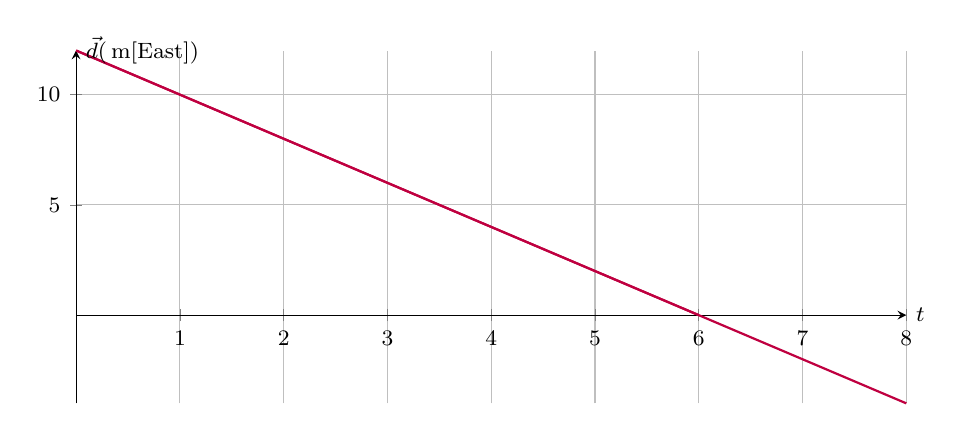
\begin{tikzpicture}
		\begin{axis}[
			my axis style,
			width=\textwidth,
			height=.5\textwidth,
			grid
		]
		
		\addplot[
			domain=0:6,
			thick,
			purple,
			-
		]
		{-2*x + 12};


		\addplot[
			domain=0:8,
			thick,
			purple,
			-
		]
		{-2*x + 12};
		
		\fill[
			black
		];
		
		\end{axis}
		\end{tikzpicture}
		\end{center}

\end{qstn}



\begin{qstn}[9]
(Half circle problem)

\end{qstn}

\begin{qstn}[10]
(Bunny hopping relative vetcor problem)
\end{qstn}

\begin{qstn}[11]
(Cliff problem)
\end{qstn}



\end{document}



















